\section{Methodology}\label{sec:Methodology}

The methodology used in this research is summarized in the flowchart in \textbf{Figure \ref{fig:CH03_Methodology}}. 

\begin{figure}[h]
    \centering
    \caption{Methodology}
    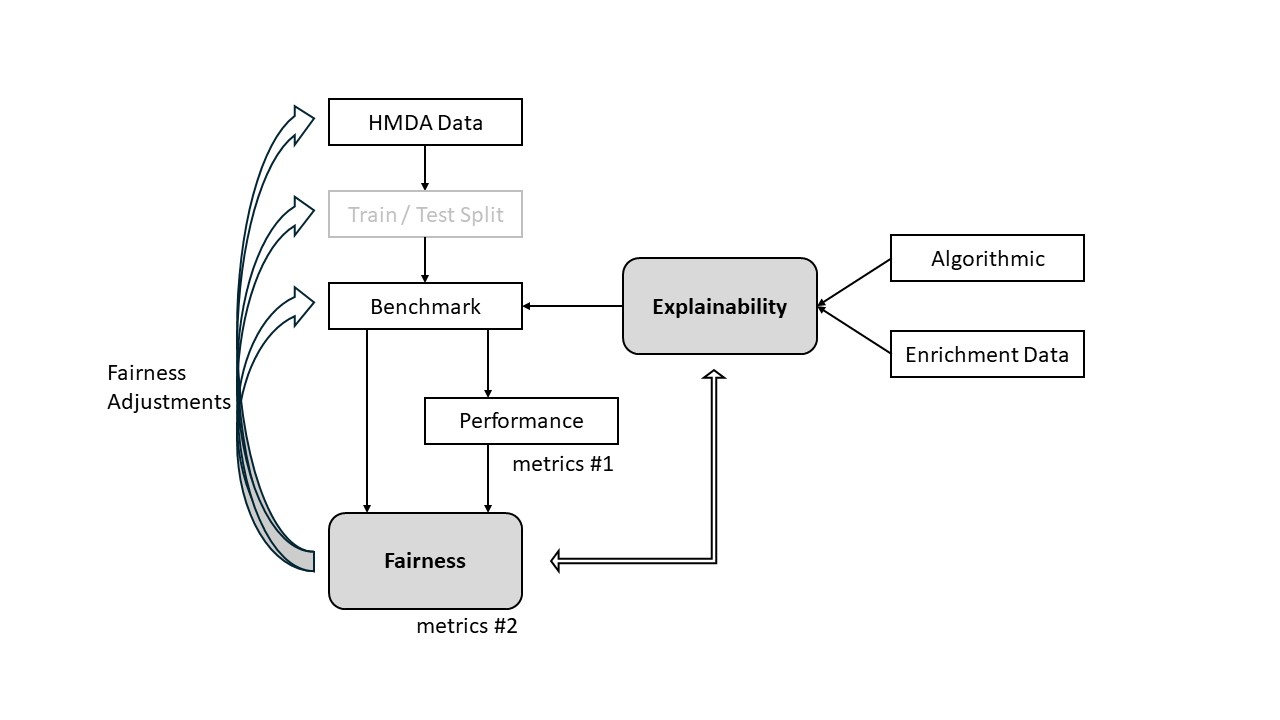
\includegraphics[width=0.85\textwidth]{CH03_Methodology.jpg}
    \caption*{The procedure chosen for this thesis follows an iterative approach: After the initial model training and prediction, explainability and performance are assessed. Based on these results, adjustments are made to the model and the data preparation process. The fairness of the model is then evaluated using the Aequitas framework. This process is repeated until a satisfactory model is achieved.}
    \label{fig:CH03_Methodology}
\end{figure}

Data Preparation and Splitting have already been discussed in \textbf{Chapter \ref{subsec:Data_Preparation}}, details on the remaining steps will be provided in the following.

\subsection{Model Training and Prediction}\label{subsec:Model_Training_and_Prediction}

The model chosen is a comparably simple sequential neural network, implemented with the keras package. Model details are provided in \textbf{Table \ref{tab:CH03_Model_Details}}.

\begin{table}[h]
    \centering
    \caption{Summary of the Neural Network}
    \begin{tabularx}{\textwidth}{lXr}
    \hline
    \textbf{Layer (type)} & \textbf{Output Shape} & \textbf{Param \#} \\
    \hline
    dense & (None, 32) & 640 \\
    dense\_1 & (None, 64) & 2112 \\
    dropout & (None, 64) & 0 \\
    dense\_2 & (None, 128) & 8320 \\
    dropout\_1 & (None, 128) & 0 \\
    dense\_3 & (None, 64) & 8256 \\
    dropout\_2 & (None, 64) & 0 \\
    dense\_4 & (None, 1) & 65 \\
    \hline
    \textbf{Total params} & & 19,393 \\
    \textbf{Trainable params} & & 19,393 \\
    \textbf{Non-trainable params} & & 0 \\
    \hline
    \end{tabularx}
    \caption*{The neural network consists of 5 dense layers (with 32, 64, 128, 64, and 1 neuron per layer), with 3 dropout layers (with dropout rates of 0.1, 0.25, and 0.1 respectively) in between. L2 regularization (0.001) is utilized in each dense layer. The total number of parameters is 19,393.}
    \label{tab:CH03_Model_Details}
\end{table}

To increase the efficiency of the training process and to prevent overfitting, \textit{callbacks} for early stopping (with a patience of 5 iterations) and best model selection, both based on the validation loss, have been implemented. 
\textit{Adam} was chosen as the optimizer, due to the nature of the classification task, loss evaluation was based on \textit{binary crossentropy}, and \textit{accuracy} was selected as the target metric. Training took place with a batch size of 48 and for a maximum of 30 epochs. 

\subsection{Explainability}\label{subsec:Explainability}

As laid out in the research question for this thesis (see \textbf{chapter \ref{ch:Introduction}}), an important part of assessing the models fairness is the ability to actually explain its decisions.
A total of three different Explainability algorithms (see \textbf{chapter\ref{subsec:algorithms}} for theoretical background) were utilized for two reasons: Firstly, to provide a comprehensive overview of the models' decision-making process, and secondly, to understand potential differences in the results of the algorithms, in case any may arise.
\begin{itemize}
    \item The \textbf{SHAP} algorithm will be applied to a set of individual predictions, aiming to understand feature importance and the impact of individual features on the model's decision.
    \item The \textbf{LIME} algorithm will be used to challenge the predictions made by the SHAP algorithms to assess whether both provide comparable explanations.
    \item A \textbf{Global Surrogate Model} will be trained on the model's prediction to assess whether the local explanations made by LIME and SHAP are also reflected on a global level.
\end{itemize}
The combination of these three algorithms aims to benefit not only model understanding, but also the analysis of potential differences in the predictions.

\subsection{Performance Assessment}\label{subsec:Performance_Assessment}

The model originally puts out numerical probabilities, which are then converted to binary values, using a threshold of 0.5.
Using these original probabilities, \textbf{ROC AUC} curves can be plotted and the ROC AUC score can be calculated, which is used as one of the assessment measures.
Additionally, a common set of classification metrics, being \textbf{accuracy}, \textbf{precision}, \textbf{recall}, and \textbf{F1 score}, are calculated alongside the \textbf{confusion matrix}.

Finding comparable benchmarks for model performance in the academic literature is hampered by the recency of the used data and the individual approach to filtering states.
Papers with a similar approach were able to achieve a ROC AUC of \textit{0.768} on a regression task \parencite{Ghoba} with somewhat comparable data, 
or reported an accuracy of 91\% using a deep neural network for classification \parencite{Hodges2024}, albeit with a different timeframe and a higher amount of used features. 

\subsection{Fairness Assessment}\label{subsec:Fairness_Assessment}

% Describe aequitas procedure
% Describe aif360 procedure(?)
% Refer to formulas from literature review (and probably move / delete them)
% Metrics: Choice of metrics, reasoning, details of application - choose most important ones from aequitas summary

Aequitas provides a multitude of fairness metrics to provide model fairness. In order to work with a uniform framework in this thesis, four easy to understand yet highly relevant metrics are chosen: 
The disparities in \textbf{False Positive Rate} (FPR) and \textbf{False Negative Rate} (FNR), as well as the \textbf{True Positive Rate} (TPR) and \textbf{True Negative Rate} (TNR) are calculated for the different groups.
Analyzing these will inform about how much more likely the model is to make one of the four predictions for Black or African American Americans compared to White applicants.
From the original paper \parencite{2018aequitas}, we can infer these formulas for the calculation of the disparities:

\begin{equation}
    FPR_{g_{\text{disp}}} = \frac{FPR_{a_i}}{FPR_{a_r}} = \frac{\Pr(\hat{Y}=1 | Y=0, A=a_i)}{\Pr(\hat{Y}=1 | Y=0, A=a_r)}
    \label{eq:FPR_Disparity}
    \addcontentsline{frm}{formulas}{\protect\numberline{\theequation}\hspace{1em}FPR Disparity}
\end{equation}

\begin{equation}
    FNR_{g_{\text{disp}}} = \frac{FNR_{a_i}}{FNR_{a_r}} = \frac{\Pr(\hat{Y}=0 | Y=1, A=a_i)}{\Pr(\hat{Y}=0 | Y=1, A=a_r)}
    \label{eq:FNR_Disparity}
    \addcontentsline{frm}{formulas}{\protect\numberline{\theequation}\hspace{1em}FNR Disparity}
\end{equation}

\begin{equation}
    TPR_{g_{\text{disp}}} = \frac{TPR_{a_i}}{TPR_{a_r}} = \frac{\Pr(\hat{Y}=1 | Y=1, A=a_i)}{\Pr(\hat{Y}=1 | Y=1, A=a_r)}
    \label{eq:TPR_Disparity}
    \addcontentsline{frm}{formulas}{\protect\numberline{\theequation}\hspace{1em}TPR Disparity}
\end{equation}

\begin{equation}
    TNR_{g_{\text{disp}}} = \frac{TNR_{a_i}}{TNR_{a_r}} = \frac{\Pr(\hat{Y}=0 | Y=0, A=a_i)}{\Pr(\hat{Y}=0 | Y=0, A=a_r)}
    \label{eq:TNR_Disparity}
    \addcontentsline{frm}{formulas}{\protect\numberline{\theequation}\hspace{1em}TNR Disparity}
\end{equation}

Following the original paper, the optimal value for the disparities is \textbf{1}, as this would indicate parity between the groups. This means, that increased fairness is indicated by values closer to \textbf{1} when comparing model results to each other.

% Add a more specific analysis of e.g. subgroup precision etc.

\subsection{Explainability and Fairness through Enrichment Data}\label{subsec:Enrichment_Data_Methodology}

An additional approach to Explainability is the use of geographical data (see \textbf{chapter \ref{subsec:Enrichment_Data}}). As the dataset contains information on the geographical location of the applicants, it was possible to analyze the distribution of granted loans across different regions by joining the mortgage data to economic variables of the corresponding regions using FIPS identifiers. 
While this procedure does not build upon the usage of an Explainability algorithm per se, it does support the understanding of the model's decision-making process (thereby addressing both explainability and fairness concerns) by providing additional context that might not be directly grasped from the data itself.

In order to operationalize this approach, the following steps were taken:
\begin{itemize}
    \item The data was aggregated on \textit{county\_code} level, using the \textit{groupby} function of the pandas package.
    \item Aggregated KPIs were created: 
    \begin{itemize}
        \item \textbf{Sum of Applications}: The total number of applications per county, mainly important to filter out counties with a low number of applications.
        \item \textbf{Percentage of Grants}: The overall likelihood of a positive decision per county.
        \item \textbf{Percentage White Applicants}: The percentage of White applicants per county.
    \end{itemize}
    \item These KPIs were then related to the predictions made by the model by creating the \textbf{Perc. Pred. Grants} feature, which is the percentage of granted loans per county predicted by the model.
    \item Based on this set of information, several scatterplots relating these factors were created to analyze the distribution of granted loans across different regions, incorporating information on potentially discriminating factors. 
\end{itemize}

\subsection{Iterations}\label{subsec:Iterations}

% Maybe more detail when decision has actually been made?
% Workflow idea: Training (unadjusted) -> Explainability -> Performance -> Fairness by using aequitas outcome (or checking AIF360) -> new technique by AIF 360 -> aim for similar performance but better fairness

Based on the results of the performance and fairness assessments for the initial model run (see \textbf{Chapter \ref{subsec:Iteration_I}}), adjustments to the model and the data preparation process were made in multiple iterations, aiming to improve at least one of these aspects in each run.

As a first iteration, \textbf{Reweighing} was applied. This \textit{pre-processing} procedure was initially developed by Calders et al. \parencite{Calders2009} and is implemented in the \textbf{AIF360} package. It works by adding a weight to each sample in the training data with the aim of balancing the weights of the different groups without actually adjusting any values.
The practical application of this technique includes the following steps: Initially, the weights of the samples need to be calculated. This can be achieved using the \textit{Reweighing} class of the \textit{aif360.algorithms.preprocessing} module. Being supplied with the training dataset and information on the privileged group (in this case, the \textit{White} applicants) and the unprivileged group (\textit{Black and African American} applicants), the algorithm calculates the weights for each sample. 
In order to ensure comparability of the results, an exact copy of the neural network described in \textbf{Figure \ref{tab:CH03_Model_Details}} is created and compiled. During fitting however, the weights calculated by the reweighing algorithm are passed to the \textit{sample\_weight} parameter of the model, causing keras to apply them during model fitting. The results of this iteration can be found in \textbf{Chapter \ref{subsec:Iteration_I}}.

The second iteration consisted of the application of the \textbf{Correlation Remover}, another pre-processing technique that was proposed by Weerts et al.\ in their paper on the Fairlearn Python package \parencite{Weerts2023}. It aims to remove any correlation between the sensitive attribute and the features of the dataset, while changes in non-sensitive features are kept as low as possible:

\begin{equation}
    \begin{aligned}
        & \underset{z_1, \ldots, z_n}{\text{min}}
        & & \sum_{i=1}^n ||z_i - x_i||^2 \\
        & \text{subject to}
        & & \frac{1}{n} \sum_{i=1}^n z_i (s_i - \bar{s})^T = 0
        \end{aligned}
    \label{eq:Correlation_Remover}
    \addcontentsline{frm}{formulas}{\protect\numberline{\theequation}\hspace{1em}Correlation Remover}
\end{equation}

Practically implementing this technique requires a definition of the sensitive attribute $s$ (as opposed to non-sensitive attributes $z$), which will then be used to fulfill the constraint of the optimization problem as displayed in \textbf{equation \ref{eq:Correlation_Remover}}. 
Once again, the neural network needs to be retrained on the dataset after the application of the Correlation Remover. It must however be noted, that, as opposed to the reweighing technique, the underlying data are actually altered by this technique, meaning that a model fitted on correlation-removed data will only perform well on correlation-removed validation and testing data. The results of this iteration can be found in \textbf{chapter \ref{subsec:Iteration_II}}.

As a third iteration, a post-processing technique was applied: The \textbf{Calibrated Equalized Odds Postprocessing} algorithm, initially proposed by Pleiss et al. \parencite{Pleiss2017}. It aims to satisfy the \textit{Equalized Odds} criterion (see \textbf{chapter \ref{subsec:overview}}) while keeping the results \textit{calibrated}, i.e. making sure that the predictions probabilities are interpretable as levels of confidence.
This algorithm has been implemented in the \textit{AIF360} package \footnote{More information on practical applications can be found under \url{https://github.com/Trusted-AI/AIF360/blob/main/examples/demo_calibrated_eqodds_postprocessing.ipynb}} and can be applied to the model's predictions after the model has been trained by transforming the data with regards to the selected fairness constraint. The results of this iteration can be found in \textbf{chapter \ref{subsec:Iteration_III}}. 

% Add reasoning for each iteration!!!